% Options for packages loaded elsewhere
\PassOptionsToPackage{unicode}{hyperref}
\PassOptionsToPackage{hyphens}{url}
\PassOptionsToPackage{dvipsnames,svgnames,x11names}{xcolor}
%
\documentclass[
  letterpaper,
  DIV=11,
  numbers=noendperiod]{scrartcl}

\usepackage{amsmath,amssymb}
\usepackage{iftex}
\ifPDFTeX
  \usepackage[T1]{fontenc}
  \usepackage[utf8]{inputenc}
  \usepackage{textcomp} % provide euro and other symbols
\else % if luatex or xetex
  \usepackage{unicode-math}
  \defaultfontfeatures{Scale=MatchLowercase}
  \defaultfontfeatures[\rmfamily]{Ligatures=TeX,Scale=1}
\fi
\usepackage{lmodern}
\ifPDFTeX\else  
    % xetex/luatex font selection
\fi
% Use upquote if available, for straight quotes in verbatim environments
\IfFileExists{upquote.sty}{\usepackage{upquote}}{}
\IfFileExists{microtype.sty}{% use microtype if available
  \usepackage[]{microtype}
  \UseMicrotypeSet[protrusion]{basicmath} % disable protrusion for tt fonts
}{}
\makeatletter
\@ifundefined{KOMAClassName}{% if non-KOMA class
  \IfFileExists{parskip.sty}{%
    \usepackage{parskip}
  }{% else
    \setlength{\parindent}{0pt}
    \setlength{\parskip}{6pt plus 2pt minus 1pt}}
}{% if KOMA class
  \KOMAoptions{parskip=half}}
\makeatother
\usepackage{xcolor}
\setlength{\emergencystretch}{3em} % prevent overfull lines
\setcounter{secnumdepth}{-\maxdimen} % remove section numbering
% Make \paragraph and \subparagraph free-standing
\makeatletter
\ifx\paragraph\undefined\else
  \let\oldparagraph\paragraph
  \renewcommand{\paragraph}{
    \@ifstar
      \xxxParagraphStar
      \xxxParagraphNoStar
  }
  \newcommand{\xxxParagraphStar}[1]{\oldparagraph*{#1}\mbox{}}
  \newcommand{\xxxParagraphNoStar}[1]{\oldparagraph{#1}\mbox{}}
\fi
\ifx\subparagraph\undefined\else
  \let\oldsubparagraph\subparagraph
  \renewcommand{\subparagraph}{
    \@ifstar
      \xxxSubParagraphStar
      \xxxSubParagraphNoStar
  }
  \newcommand{\xxxSubParagraphStar}[1]{\oldsubparagraph*{#1}\mbox{}}
  \newcommand{\xxxSubParagraphNoStar}[1]{\oldsubparagraph{#1}\mbox{}}
\fi
\makeatother

\usepackage{color}
\usepackage{fancyvrb}
\newcommand{\VerbBar}{|}
\newcommand{\VERB}{\Verb[commandchars=\\\{\}]}
\DefineVerbatimEnvironment{Highlighting}{Verbatim}{commandchars=\\\{\}}
% Add ',fontsize=\small' for more characters per line
\usepackage{framed}
\definecolor{shadecolor}{RGB}{241,243,245}
\newenvironment{Shaded}{\begin{snugshade}}{\end{snugshade}}
\newcommand{\AlertTok}[1]{\textcolor[rgb]{0.68,0.00,0.00}{#1}}
\newcommand{\AnnotationTok}[1]{\textcolor[rgb]{0.37,0.37,0.37}{#1}}
\newcommand{\AttributeTok}[1]{\textcolor[rgb]{0.40,0.45,0.13}{#1}}
\newcommand{\BaseNTok}[1]{\textcolor[rgb]{0.68,0.00,0.00}{#1}}
\newcommand{\BuiltInTok}[1]{\textcolor[rgb]{0.00,0.23,0.31}{#1}}
\newcommand{\CharTok}[1]{\textcolor[rgb]{0.13,0.47,0.30}{#1}}
\newcommand{\CommentTok}[1]{\textcolor[rgb]{0.37,0.37,0.37}{#1}}
\newcommand{\CommentVarTok}[1]{\textcolor[rgb]{0.37,0.37,0.37}{\textit{#1}}}
\newcommand{\ConstantTok}[1]{\textcolor[rgb]{0.56,0.35,0.01}{#1}}
\newcommand{\ControlFlowTok}[1]{\textcolor[rgb]{0.00,0.23,0.31}{\textbf{#1}}}
\newcommand{\DataTypeTok}[1]{\textcolor[rgb]{0.68,0.00,0.00}{#1}}
\newcommand{\DecValTok}[1]{\textcolor[rgb]{0.68,0.00,0.00}{#1}}
\newcommand{\DocumentationTok}[1]{\textcolor[rgb]{0.37,0.37,0.37}{\textit{#1}}}
\newcommand{\ErrorTok}[1]{\textcolor[rgb]{0.68,0.00,0.00}{#1}}
\newcommand{\ExtensionTok}[1]{\textcolor[rgb]{0.00,0.23,0.31}{#1}}
\newcommand{\FloatTok}[1]{\textcolor[rgb]{0.68,0.00,0.00}{#1}}
\newcommand{\FunctionTok}[1]{\textcolor[rgb]{0.28,0.35,0.67}{#1}}
\newcommand{\ImportTok}[1]{\textcolor[rgb]{0.00,0.46,0.62}{#1}}
\newcommand{\InformationTok}[1]{\textcolor[rgb]{0.37,0.37,0.37}{#1}}
\newcommand{\KeywordTok}[1]{\textcolor[rgb]{0.00,0.23,0.31}{\textbf{#1}}}
\newcommand{\NormalTok}[1]{\textcolor[rgb]{0.00,0.23,0.31}{#1}}
\newcommand{\OperatorTok}[1]{\textcolor[rgb]{0.37,0.37,0.37}{#1}}
\newcommand{\OtherTok}[1]{\textcolor[rgb]{0.00,0.23,0.31}{#1}}
\newcommand{\PreprocessorTok}[1]{\textcolor[rgb]{0.68,0.00,0.00}{#1}}
\newcommand{\RegionMarkerTok}[1]{\textcolor[rgb]{0.00,0.23,0.31}{#1}}
\newcommand{\SpecialCharTok}[1]{\textcolor[rgb]{0.37,0.37,0.37}{#1}}
\newcommand{\SpecialStringTok}[1]{\textcolor[rgb]{0.13,0.47,0.30}{#1}}
\newcommand{\StringTok}[1]{\textcolor[rgb]{0.13,0.47,0.30}{#1}}
\newcommand{\VariableTok}[1]{\textcolor[rgb]{0.07,0.07,0.07}{#1}}
\newcommand{\VerbatimStringTok}[1]{\textcolor[rgb]{0.13,0.47,0.30}{#1}}
\newcommand{\WarningTok}[1]{\textcolor[rgb]{0.37,0.37,0.37}{\textit{#1}}}

\providecommand{\tightlist}{%
  \setlength{\itemsep}{0pt}\setlength{\parskip}{0pt}}\usepackage{longtable,booktabs,array}
\usepackage{calc} % for calculating minipage widths
% Correct order of tables after \paragraph or \subparagraph
\usepackage{etoolbox}
\makeatletter
\patchcmd\longtable{\par}{\if@noskipsec\mbox{}\fi\par}{}{}
\makeatother
% Allow footnotes in longtable head/foot
\IfFileExists{footnotehyper.sty}{\usepackage{footnotehyper}}{\usepackage{footnote}}
\makesavenoteenv{longtable}
\usepackage{graphicx}
\makeatletter
\newsavebox\pandoc@box
\newcommand*\pandocbounded[1]{% scales image to fit in text height/width
  \sbox\pandoc@box{#1}%
  \Gscale@div\@tempa{\textheight}{\dimexpr\ht\pandoc@box+\dp\pandoc@box\relax}%
  \Gscale@div\@tempb{\linewidth}{\wd\pandoc@box}%
  \ifdim\@tempb\p@<\@tempa\p@\let\@tempa\@tempb\fi% select the smaller of both
  \ifdim\@tempa\p@<\p@\scalebox{\@tempa}{\usebox\pandoc@box}%
  \else\usebox{\pandoc@box}%
  \fi%
}
% Set default figure placement to htbp
\def\fps@figure{htbp}
\makeatother

\KOMAoption{captions}{tableheading}
\makeatletter
\@ifpackageloaded{caption}{}{\usepackage{caption}}
\AtBeginDocument{%
\ifdefined\contentsname
  \renewcommand*\contentsname{Table of contents}
\else
  \newcommand\contentsname{Table of contents}
\fi
\ifdefined\listfigurename
  \renewcommand*\listfigurename{List of Figures}
\else
  \newcommand\listfigurename{List of Figures}
\fi
\ifdefined\listtablename
  \renewcommand*\listtablename{List of Tables}
\else
  \newcommand\listtablename{List of Tables}
\fi
\ifdefined\figurename
  \renewcommand*\figurename{Figure}
\else
  \newcommand\figurename{Figure}
\fi
\ifdefined\tablename
  \renewcommand*\tablename{Table}
\else
  \newcommand\tablename{Table}
\fi
}
\@ifpackageloaded{float}{}{\usepackage{float}}
\floatstyle{ruled}
\@ifundefined{c@chapter}{\newfloat{codelisting}{h}{lop}}{\newfloat{codelisting}{h}{lop}[chapter]}
\floatname{codelisting}{Listing}
\newcommand*\listoflistings{\listof{codelisting}{List of Listings}}
\makeatother
\makeatletter
\makeatother
\makeatletter
\@ifpackageloaded{caption}{}{\usepackage{caption}}
\@ifpackageloaded{subcaption}{}{\usepackage{subcaption}}
\makeatother

\usepackage{bookmark}

\IfFileExists{xurl.sty}{\usepackage{xurl}}{} % add URL line breaks if available
\urlstyle{same} % disable monospaced font for URLs
\hypersetup{
  pdftitle={projetSeriTemp},
  pdfauthor={Saïdou YAMEOGO},
  colorlinks=true,
  linkcolor={blue},
  filecolor={Maroon},
  citecolor={Blue},
  urlcolor={Blue},
  pdfcreator={LaTeX via pandoc}}


\title{projetSeriTemp}
\author{Saïdou YAMEOGO}
\date{}

\begin{document}
\maketitle


\section{\texorpdfstring{Sujet de recherche : \textbf{\emph{Modélisation
économétrique de la production de coton au Burkina Faso : une analyse en
séries temporelles de l'impact des précipitations, des prix à
l'exportation et des subventions publiques
(1990--2023)}}}{Sujet de recherche : Modélisation économétrique de la production de coton au Burkina Faso : une analyse en séries temporelles de l'impact des précipitations, des prix à l'exportation et des subventions publiques (1990--2023)}}\label{sujet-de-recherche-moduxe9lisation-uxe9conomuxe9trique-de-la-production-de-coton-au-burkina-faso-une-analyse-en-suxe9ries-temporelles-de-limpact-des-pruxe9cipitations-des-prix-uxe0-lexportation-et-des-subventions-publiques-19902023}

\section{Introduction}\label{introduction}

Au cœur de l'économie burkinabè, le coton occupe une place stratégique,
tant par son poids dans les exportations que par son rôle dans les
revenus des ménages ruraux. Depuis les années 1960, cette culture de
rente n'a cessé de façonner l'organisation agricole, les politiques
publiques et les dynamiques commerciales du pays. Le Burkina Faso s'est
ainsi hissé au rang de premier producteur de coton en Afrique de l'Ouest
pendant plusieurs décennies, avant de connaître des fluctuations
marquées dans sa production.

Ces variations soulèvent une interrogation essentielle : quels sont les
véritables moteurs de la production cotonnière au Burkina Faso ? En
effet, si la volonté des producteurs est incontestable, les rendements
demeurent sensibles à des facteurs externes tels que les conditions
climatiques, la volatilité des prix internationaux, ou encore le soutien
financier de l'État.

Dans un contexte mondial marqué par le changement climatique,
l'instabilité des marchés et la pression sur les finances publiques, il
devient crucial d'analyser ces trois leviers -- les précipitations, les
prix à l'exportation et les subventions publiques -- pour comprendre
leur impact réel sur la performance cotonnière nationale. Une telle
compréhension permettrait non seulement d'améliorer la planification des
politiques agricoles, mais aussi de renforcer la résilience du secteur
face aux chocs externes.

C'est dans cette optique que s'inscrit ce travail, qui propose une
modélisation économétrique de la production de coton au Burkina Faso sur
la période 1973--2024, en mobilisant les outils des séries temporelles.
En croisant données climatiques, économiques et institutionnelles, cette
étude vise à révéler les interactions profondes entre les variables
explicatives retenues et l'évolution de la production cotonnière, afin
d'en tirer des enseignements pour les décennies à venir.

\section{Contexte et Justification}\label{contexte-et-justification}

\subsection{Contexte}\label{contexte}

Au Burkina Faso, le coton constitue l'un des piliers du secteur agricole
et de l'économie nationale. Il représente la principale culture de
rente, mobilisant plus de \textbf{350 000 producteurs} et occupant une
\textbf{place dominante dans les exportations nationales}, avec une
contribution estimée à \textbf{plus de 60 \% des recettes en devises} au
cours de certaines années. Cette filière est aussi un moteur de
développement local, notamment dans les régions de l'ouest et du
sud-ouest du pays, zones historiquement les plus productives.

La culture du coton repose essentiellement sur l'agriculture pluviale,
ce qui la rend particulièrement vulnérable aux \textbf{variations
climatiques}, notamment aux aléas pluviométriques. Dans un contexte de
\textbf{changements climatiques croissants}, la régularité et
l'intensité des précipitations deviennent de plus en plus imprévisibles,
affectant la stabilité des rendements agricoles.

En parallèle, la \textbf{libéralisation de la filière} intervenue dans
les années 2000 a modifié les mécanismes de régulation des prix et
d'accès aux intrants. L'État et ses partenaires ont mis en place
diverses politiques d'appui à travers des \textbf{subventions
agricoles}, la \textbf{structuration des sociétés cotonnières} (SOFITEX,
Faso Coton, SOCOMA), et la création du \textbf{fonds de lissage} pour
atténuer les effets de la volatilité des prix sur les producteurs.

Enfin, le \textbf{marché international du coton} est particulièrement
instable. La \textbf{variation des prix à l'exportation}, influencée par
les cours mondiaux, le taux de change, et la concurrence internationale,
impacte fortement les revenus agricoles et les décisions de culture.

\subsection{Justification}\label{justification}

Le choix de ce thème s'inscrit dans une volonté de mieux
\textbf{comprendre les mécanismes structurels} qui influencent la
production cotonnière au Burkina Faso sur une période longue
(1990--2023). En effet :

\begin{itemize}
\tightlist
\item
  \textbf{Sur le plan scientifique}, peu d'études ont adopté une
  \textbf{approche économétrique en séries temporelles} pour analyser
  conjointement les effets des variables climatiques, économiques et
  institutionnelles sur la production cotonnière. Une telle analyse
  permet de prendre en compte les dynamiques de long terme, les effets
  retardés et les interdépendances structurelles.
\end{itemize}

\begin{itemize}
\tightlist
\item
  \textbf{Sur le plan politique}, une meilleure compréhension des
  déterminants de la production peut aider à orienter les politiques
  agricoles vers des mécanismes de soutien plus efficaces et adaptés aux
  nouvelles réalités climatiques et économiques.
\end{itemize}

\begin{itemize}
\tightlist
\item
  \textbf{Sur le plan économique et social}, dans un pays où une large
  part de la population dépend directement de l'agriculture, et du coton
  en particulier, une amélioration de la performance de cette filière a
  un impact direct sur \textbf{la sécurité alimentaire, les revenus des
  ménages ruraux et la réduction de la pauvreté}.
\end{itemize}

\section{Problématique}\label{probluxe9matique}

Le Burkina Faso, pays à vocation essentiellement agricole, a longtemps
tiré une part importante de ses recettes d'exportation du coton,
surnommé ``l'or blanc''. Cette culture représente non seulement une
source majeure de revenus pour des milliers de producteurs ruraux, mais
aussi un levier clé pour la croissance économique nationale. Pourtant,
malgré son rôle stratégique, la production cotonnière au Burkina Faso
demeure instable et vulnérable aux aléas de plusieurs facteurs.

D'une part, les conditions climatiques, notamment les précipitations,
influencent fortement les rendements agricoles dans un pays marqué par
une agriculture pluviale.

D'autre part, les variations des prix mondiaux du coton exposent les
producteurs aux incertitudes du marché international. Enfin, les
subventions publiques allouées au secteur (intrants, prix d'achat,
infrastructures) apparaissent comme un mécanisme d'amortissement, mais
leur régularité et leur efficacité posent également question.

Dans ce contexte, une interrogation centrale se pose : Dans quelle
mesure les précipitations, les prix à l'exportation du coton et les
subventions publiques influencent-ils la production cotonnière au
Burkina Faso entre 1990 et 2023 ?

Autrement dit, quelles sont les relations de court et de long terme
entre ces variables, et comment peuvent-elles éclairer les choix de
politiques agricoles à venir ?

\section{Revue de littérature}\label{revue-de-littuxe9rature}

La production cotonnière au Burkina Faso, culture de rente par
excellence, est soumise à plusieurs facteurs exogènes, notamment les
aléas climatiques. Contrairement à d'autres cultures pluviales, le coton
a montré une certaine résilience à travers la mise en lumière de
certaines recherches clés~:

\begin{itemize}
\item
  L'étude de \textbf{Albergel, Carbonnel et Vaugelade (1985)} met en
  évidence une forte corrélation entre la pluviométrie et la production
  cotonnière. Cette étude met également en lumière les facteurs
  climatiques et institutionnels qui influencent la production
  cotonnière au Burkina Faso. Toutefois, elle souffre d'un manque
  d'intégration dynamique et temporelle.
\item
  L'utilisation des modèles VAR pour analyser les déterminants de la
  production agricole est une approche bien établie. Yameogo (2019) a
  par exemple utilisé un modèle VAR pour analyser les effets des
  variables climatiques et économiques sur la production de maïs au
  Burkina Faso. Ce modèle permet de capturer les relations dynamiques et
  interdépendantes entre plusieurs variables économiques et climatiques
  sur de longues périodes. En ce sens, il est adapté à l'analyse de la
  production agricole, où les variables influencent et sont influencées
  les unes par les autres de manière simultanée.Les avantages de cette
  approche sont évidents, notamment sa capacité à capturer des effets de
  rétroaction entre les variables. Cependant, le modèle VAR présente
  certaines limites. Il est sensible à la sélection des variables et à
  la longueur de la période d'étude, ce qui peut mener à des résultats
  erronés si des variables clés sont omises ou si des ruptures
  structurelles se produisent dans la série temporelle. De plus, ce
  modèle peut être coûteux en termes de données et de calculs pour de
  longues séries temporelles comme celles du Burkina Faso.
\item
  Une autre approche économétrique couramment utilisée pour l'analyse
  des séries temporelles en agriculture est le modèle ARDL. Diop et
  al.~(2014) ont utilisé cette méthode pour étudier les relations à long
  terme entre les variables économiques et climatiques dans le secteur
  agricole, avec un accent particulier sur la production de coton en
  Afrique de l'Ouest. Le modèle ARDL est particulièrement adapté aux
  séries temporelles avec des variables de nature stationnaire et non
  stationnaire, ce qui est souvent le cas dans les études agricoles. Le
  principal avantage du modèle ARDL réside dans sa flexibilité, car il
  permet de traiter des séries temporelles de différents ordres de
  stationnarité sans avoir besoin de les transformer au préalable.
  Cependant, l'un des défis de cette approche est qu'elle peut
  sous-estimer les effets à court terme ou négliger l'impact de certains
  facteurs exogènes, comme les chocs mondiaux ou les crises économiques,
  qui peuvent également affecter la production de coton.
\end{itemize}

\section{Méthodologie}\label{muxe9thodologie}

\subsection{Présentation du modèle}\label{pruxe9sentation-du-moduxe8le}

Nous présenterons respectivement le modèle retenu, la définition des
variables et la formulation des hypothèses de recherche.

\begin{enumerate}
\def\labelenumi{\arabic{enumi}.}
\item
  Le Modèle retenu

  Notre étude portant sur l'analyse de l'impact des subventions, des
  \textbf{précipitations, des prix à l'exportation et les superficies
  allouées à la culture du coton sur la production du coton a}u Burkina
  via les chocs sur ces variables, nous appréhendons l'effet a travers
  le Modèle ARIMAX( f ).

  Le modèle ARIMAX (AutoRegressive Integrated Moving Average with
  eXogenous inputs) est une version avancée du modèle ARIMA
  (AutoRegressive Integrated Moving Average). Il étend le cadre ARIMA en
  intégrant des variables exogènes, c'est-à-dire des facteurs externes
  susceptibles d'influencer la série chronologique étudiée. Cette
  intégration permet au modèle d'exploiter des informations
  supplémentaires susceptibles d'améliorer considérablement la
  précision~des~prévisions.
\item
  Choix et définition des variables

  Le modèle comporte 5 variables :

  \textbf{production :} représente la production totale du coton au
  Burkina par saison. Cette variable est cruciale dans notre étude car
  c'est elle la variable dependante ( Celle qu'on cherche à expliquer ).
  Elle est exprimée en tonnes de coton.

  \textbf{surperficie} : cette variable représente la surface totale
  allouée à la culture du coton par saison; elle est exprimée en hectare
  (ha)

  La considération de cette variable dans notre modèle s'explique par le
  fait que la production du coton depend de la superficie allouée pour
  la production.

  \textbf{prix} : cette variable désigne le prix (en franc CFA ) du kg
  de coton du prémier choix au Burkina retardé d'une année. En effet ce
  retardement va nous permettre d'analyse l'effet du prix enterieur
  (celui de l'année passée ) sur la production actuelle.

  \textbf{subvention} : cette variable représente la subvention que le
  gouvernement accorde au secteur cotonnier du pays. Elle est en
  millions de FCFA. Cette variable nous permettra de comprendre l'impact
  de la subvention sur la production du coton.

  \textbf{précipitation} : cette variable désigne la quantité moyenne de
  precipitation enregistrée durant la saison de production mesurée en
  mm. Cette variable cruciale dans notre modèle du fait que la
  production cotonnière du pays depend de la pluviométrie uniquement.
\item
  Sources des données et hypothèse de recherche

  3.1. Sources de données

  La présente étude porte sur des données annuelles s'étalant entre 1990
  et 2023 ; c'est à dire 34 observations. Les données utilisées dans le
  cadre de cette étude sont des données secondaires, tirées sur des
  bases de données existantes ou dans des journaux spécialisés. Les
  variables retenues viennent alors de diverses sources, ainsi :

  - Les productions, les superficies, les données climatiques , les prix
  du coton de 2013 à 2022 viennent du site open data du Burkina Faso (
  \url{https://burkinafaso.opendataforafrica.org/} )

  - Les prix du coton : le reste des données sont collectées dans des
  articles de presse comme faso.net, le sidwaya et dans le site officiel
  de SOFITEX

  - Les subventions : les données allant de 2006 à 2013 sont collectées
  sur :
  \url{https://openknowledge.fao.org/server/api/core/bitstreams/af7b59a7-ba8f-4da0-87f9-4a361f1ef6f0/content?utm_source=chatgpt.com}
  , les données de 2014 à 2023 sont collectées dans des articles de
  presse comme faso.net, le sidwaya et le site officiel de SOFITEX.

  - Docummentation sur la construction du modèle VECM ( memoire en
  ligne) :
  \url{https://www.memoireonline.com/03/12/5509/Impact-des-subventions-agricoles-sur-les-exportations-de-coton-du-Burkina-Faso.html?utm_source=chatgpt.com}

  \paragraph{3.2 Hypothèse de
  recherche}\label{hypothuxe8se-de-recherche}

  Nous avons posé les hypothèses de recherche suivantes :

  \textbf{Hypothèse} : Les subventions, les superficie allouées à la
  production du coton, le prix anterieur du coton et la pluviometrie
  impactent positivement sur la production du coton du Burkina. En
  d'autre terme l'augmentations des subventions de l'Etat sur la culture
  du coton contribue à augmenter la production du coton. De même
  l'augmentation des superficies allouées a la production du coton tend
  à accroitre la production cotonnière. Plus le prix de l'année
  précédente est élevée, plus les producteurs auront tendance à produire
  encore plus. Etant donné que la production de coton dépend de la
  pluviométrie, une forte précipitation peut contribuer à accroitre la
  production.
\end{enumerate}

\subsection{Méthode d'analyse et interprétation des résultats de
simulation}\label{muxe9thode-danalyse-et-interpruxe9tation-des-ruxe9sultats-de-simulation}

Cette section sera consacrée d'abord à la statistique descriptive de nos
données et leurs visualisations pour apprehender la tendance globale
puis la méthode d'analyse qui consistera à un test de diagnostic sur les
données du modèle. Ensuite nous aborderons l'estimation du modèle
ARIMAX. Et en fin nous interpréterons les résultats de simulation, qui
consisteront à une interprétation des fonctions de réponse
impulsionnelles et de la décomposition de la variance.

\begin{enumerate}
\def\labelenumi{\arabic{enumi}.}
\item
  La Statistique descriptive et la visualisation

  \begin{itemize}
  \tightlist
  \item
    Statistiques describtives de base
  \end{itemize}

\begin{Shaded}
\begin{Highlighting}[]
\CommentTok{\#| echo: False}

\NormalTok{dff}\OtherTok{\textless{}{-}}\NormalTok{  df }\SpecialCharTok{\%\textgreater{}\%}
  \FunctionTok{select}\NormalTok{(}\SpecialCharTok{{-}}\NormalTok{date)}

\NormalTok{desc\_table }\OtherTok{\textless{}{-}}\NormalTok{ dff }\SpecialCharTok{\%\textgreater{}\%}
  \FunctionTok{summarise}\NormalTok{(}\FunctionTok{across}\NormalTok{(}
    \FunctionTok{everything}\NormalTok{(),}
    \FunctionTok{list}\NormalTok{(}
      \AttributeTok{mean =} \SpecialCharTok{\textasciitilde{}}\FunctionTok{mean}\NormalTok{(., }\AttributeTok{na.rm =} \ConstantTok{TRUE}\NormalTok{),}
      \AttributeTok{median =} \SpecialCharTok{\textasciitilde{}}\FunctionTok{median}\NormalTok{(., }\AttributeTok{na.rm =} \ConstantTok{TRUE}\NormalTok{),}
      \AttributeTok{sd =} \SpecialCharTok{\textasciitilde{}}\FunctionTok{sd}\NormalTok{(., }\AttributeTok{na.rm =} \ConstantTok{TRUE}\NormalTok{),}
      \AttributeTok{min =} \SpecialCharTok{\textasciitilde{}}\FunctionTok{min}\NormalTok{(., }\AttributeTok{na.rm =} \ConstantTok{TRUE}\NormalTok{),}
      \AttributeTok{max =} \SpecialCharTok{\textasciitilde{}}\FunctionTok{max}\NormalTok{(., }\AttributeTok{na.rm =} \ConstantTok{TRUE}\NormalTok{),}
      \AttributeTok{cv =} \SpecialCharTok{\textasciitilde{}}\FunctionTok{sd}\NormalTok{(., }\AttributeTok{na.rm =} \ConstantTok{TRUE}\NormalTok{) }\SpecialCharTok{/} \FunctionTok{mean}\NormalTok{(., }\AttributeTok{na.rm =} \ConstantTok{TRUE}\NormalTok{)}
\NormalTok{    ),}
    \AttributeTok{.names =} \StringTok{"\{.col\}\_\{.fn\}"}
\NormalTok{  )) }\SpecialCharTok{\%\textgreater{}\%}
  \FunctionTok{pivot\_longer}\NormalTok{(}\AttributeTok{cols =} \FunctionTok{everything}\NormalTok{(), }\AttributeTok{names\_to =} \FunctionTok{c}\NormalTok{(}\StringTok{"Variable"}\NormalTok{, }\StringTok{"Statistique"}\NormalTok{), }\AttributeTok{names\_sep =} \StringTok{"\_"}\NormalTok{) }\SpecialCharTok{\%\textgreater{}\%}
  \FunctionTok{pivot\_wider}\NormalTok{(}\AttributeTok{names\_from =}\NormalTok{ Statistique, }\AttributeTok{values\_from =}\NormalTok{ value)}

\CommentTok{\# Afficher le tableau}
\FunctionTok{print}\NormalTok{(desc\_table)}
\end{Highlighting}
\end{Shaded}

\begin{verbatim}
# A tibble: 5 x 7
  Variable         mean   median       sd     min     max    cv
  <chr>           <dbl>    <dbl>    <dbl>   <dbl>   <dbl> <dbl>
1 production    445746. 456501   268340.   50730. 894982  0.602
2 superficie    410555. 409208.  193096.  119927  844895. 0.470
3 precipitation    997.    959.     200.     669.   1402  0.201
4 prix             196.    195       60.8     75     325  0.310
5 subvention     13636.      1.5  37879.       0  192000  2.78 
\end{verbatim}

  \begin{itemize}
  \tightlist
  \item
    Visualisation des séries
  \end{itemize}

  \pandocbounded{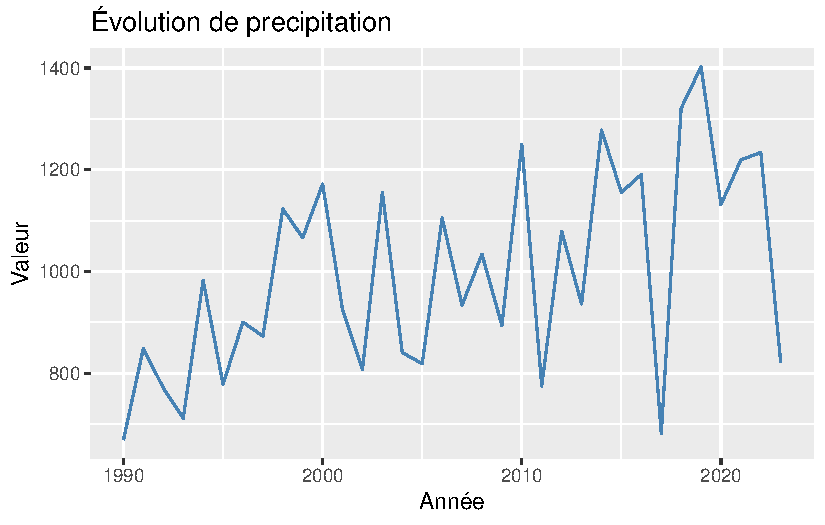
\includegraphics[keepaspectratio]{modelisation_files/figure-pdf/unnamed-chunk-4-1.pdf}}

  \pandocbounded{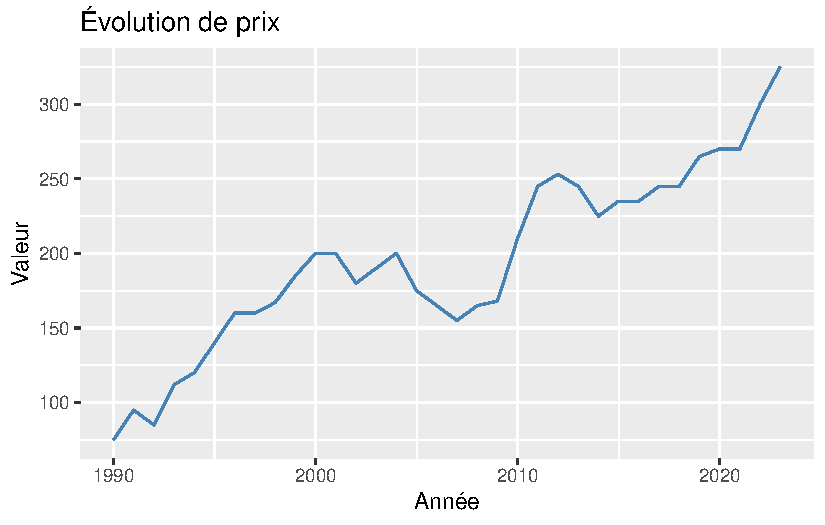
\includegraphics[keepaspectratio]{modelisation_files/figure-pdf/unnamed-chunk-4-2.pdf}}

  \pandocbounded{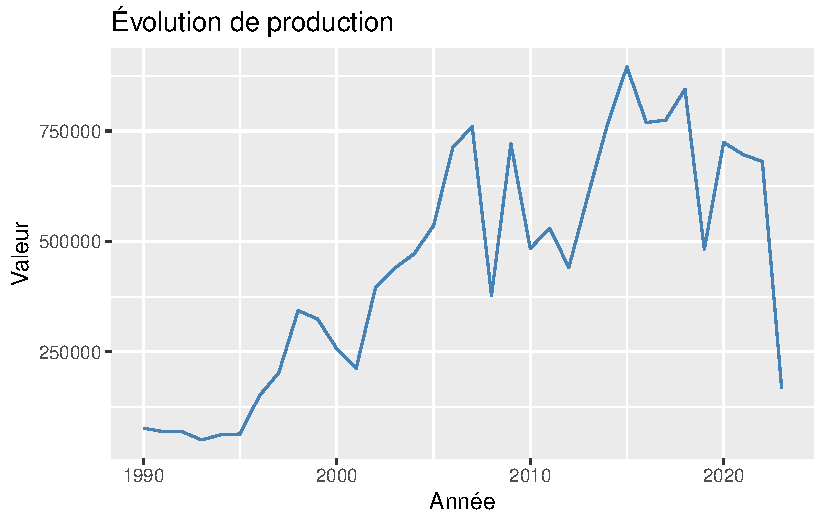
\includegraphics[keepaspectratio]{modelisation_files/figure-pdf/unnamed-chunk-4-3.pdf}}

  \pandocbounded{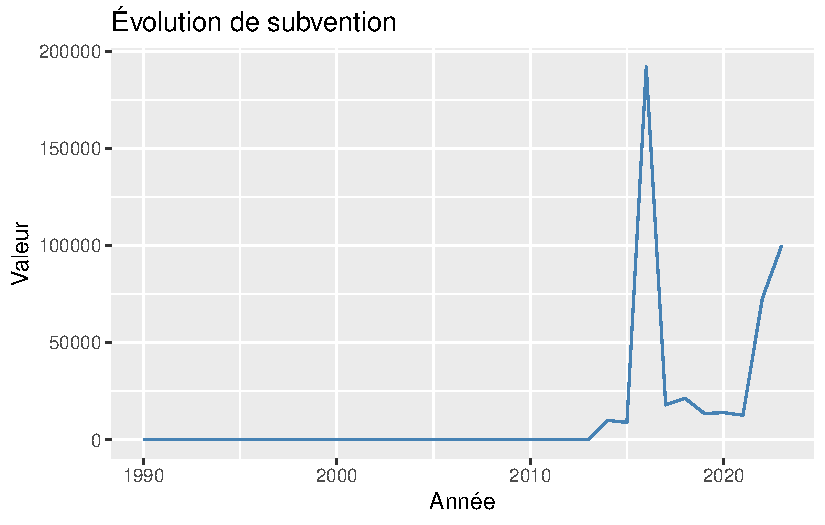
\includegraphics[keepaspectratio]{modelisation_files/figure-pdf/unnamed-chunk-4-4.pdf}}

  \pandocbounded{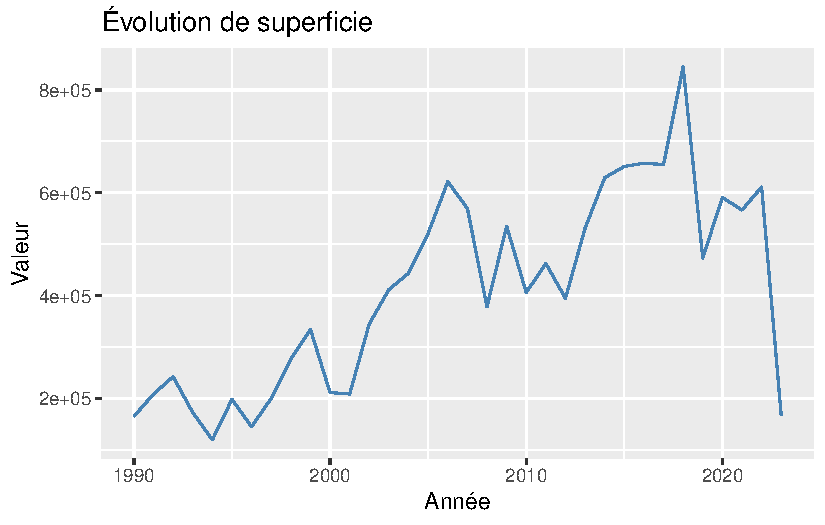
\includegraphics[keepaspectratio]{modelisation_files/figure-pdf/unnamed-chunk-4-5.pdf}}

  \pandocbounded{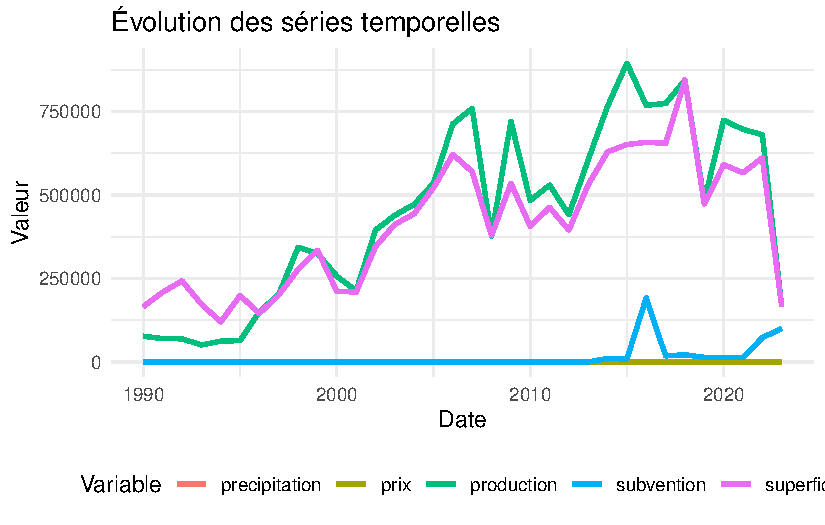
\includegraphics[keepaspectratio]{modelisation_files/figure-pdf/unnamed-chunk-5-1.pdf}}

  \begin{itemize}
  \tightlist
  \item
    La matrix de correlation
  \end{itemize}

\begin{verbatim}
              production superficie precipitation      prix subvention
production     1.0000000  0.9658617     0.5041309 0.5941711  0.2401145
superficie     0.9658617  1.0000000     0.4911324 0.5442454  0.2532747
precipitation  0.5041309  0.4911324     1.0000000 0.4976348  0.2103619
prix           0.5941711  0.5442454     0.4976348 1.0000000  0.4399864
subvention     0.2401145  0.2532747     0.2103619 0.4399864  1.0000000
\end{verbatim}

  \pandocbounded{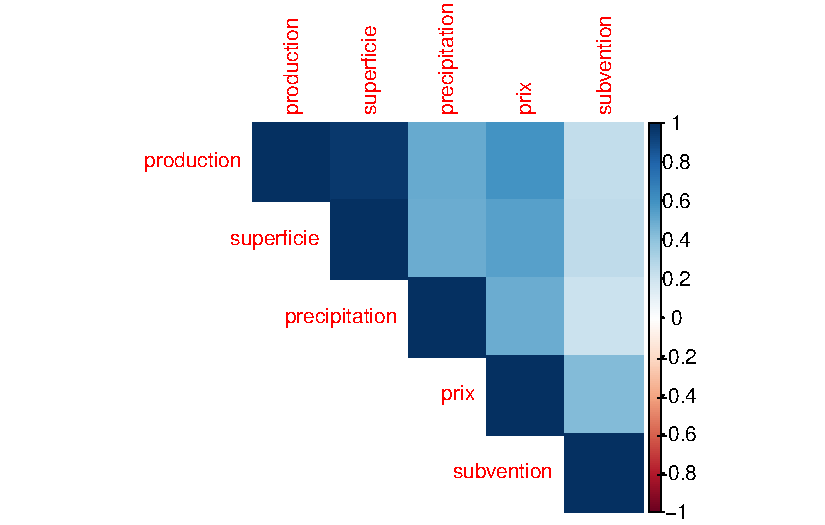
\includegraphics[keepaspectratio]{modelisation_files/figure-pdf/unnamed-chunk-6-1.pdf}}

  \begin{itemize}
  \tightlist
  \item
    Appliquons le log à notre base
  \end{itemize}

  \begin{itemize}
  \tightlist
  \item
    Reprenons la visualisation avec la fonction log
  \end{itemize}

  \pandocbounded{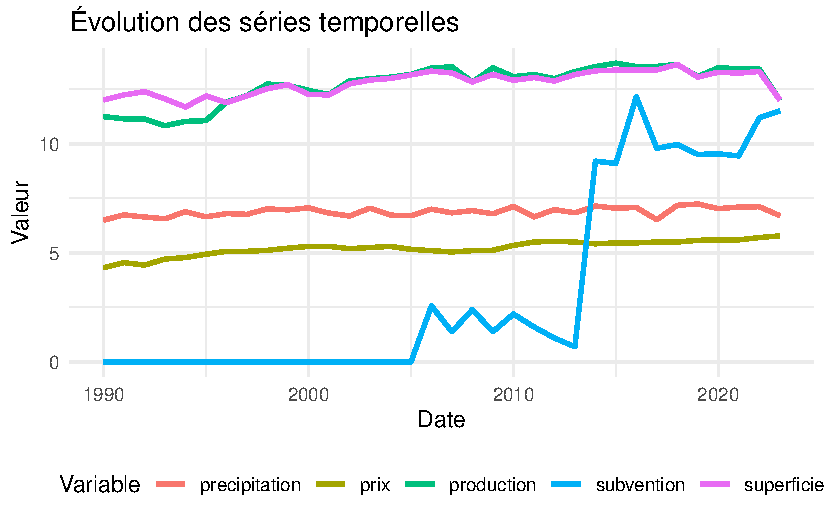
\includegraphics[keepaspectratio]{modelisation_files/figure-pdf/unnamed-chunk-8-1.pdf}}
\item
  Méthode d'analyse

  L'estimation du modèle ARIMAX nécessite un certain nombre de
  préalables. Ainsi nous commencerons par des tests de diagnostic sur
  les données avant d'estimer le modèle. Pour cela nous nous
  intéresserons à l'étude de la stationnarité des variables du modèle et
  à l'étude de leurs cointégrations.

  2.1. Etude de la stationnarité des variables :

  Depuis les travaux fondateurs de Granger et Newbold (1974) sur les
  régressions « \textbf{fallacieuses} », il convient, avant de procéder
  à des estimations sur des séries temporelles, de s'interroger au
  préalable sur la stationnarité des séries en question.

  Pour étudier la stationnarité des variables nous utilisons le test de
  Dickey- Fuller augmenté (ADF).

  Le test d'hypothèses est le suivant :

  H0: X a une racine unité (non stationnaire)

  H1: X n'a pas une racine unité (stationnaire)

  \textbf{La décision se faire comme suit} :

  Si p-value \textless{} 5\% , on rejette l'hypothèse nulle de non
  stationnarité. La série est \textbf{Stationnaire}

  Si p-value \textgreater{} 5\%, on accepte l'hypothèse nulle de non
  stationnarité. La série est \textbf{non stationnaire}

  Le test est appliqué en niveau puis en différence première puis en
  différence seconde dans le cas où les variables seraient non
  stationnaires à ces premiers stades

\begin{verbatim}
       Variable P_Value           Statut
1    production  0.9871 Non stationnaire
2    superficie  0.9802 Non stationnaire
3 precipitation  0.1991 Non stationnaire
4          prix  0.4711 Non stationnaire
5    subvention  0.1821 Non stationnaire
                                                                     Interpretation
1 La variable est non stationnaire au seuil 5% , une différenciation est nécessaire
2 La variable est non stationnaire au seuil 5% , une différenciation est nécessaire
3 La variable est non stationnaire au seuil 5% , une différenciation est nécessaire
4 La variable est non stationnaire au seuil 5% , une différenciation est nécessaire
5 La variable est non stationnaire au seuil 5% , une différenciation est nécessaire
\end{verbatim}

  Toutes les séries sont non stationnaires. Nous allons passer à la
  differenciation d'ordre 1

  \begin{itemize}
  \tightlist
  \item
    \textbf{Differenciation d'ordre 1 et test d'ADF}
  \end{itemize}

\begin{verbatim}
       Variable P_Value           Statut
1    production  0.3457 Non stationnaire
2    superficie  0.6835 Non stationnaire
3 precipitation  0.0545 Non stationnaire
4          prix  0.3913 Non stationnaire
5    subvention  0.0522 Non stationnaire
                                                                     Interpretation
1 La variable est non stationnaire au seuil 5% , une différenciation est nécessaire
2 La variable est non stationnaire au seuil 5% , une différenciation est nécessaire
3 La variable est non stationnaire au seuil 5% , une différenciation est nécessaire
4 La variable est non stationnaire au seuil 5% , une différenciation est nécessaire
5 La variable est non stationnaire au seuil 5% , une différenciation est nécessaire
\end{verbatim}

  Toutes les séries sont non stationnaires. Nous allons passer à la
  differenciation d'ordre 2

  \begin{itemize}
  \tightlist
  \item
    \textbf{Differenciation d'ordre 2 et test d'ADF}
  \end{itemize}

\begin{verbatim}
       Variable P_Value       Statut
1    production  0.0142 Stationnaire
2    superficie  0.0166 Stationnaire
3 precipitation  0.0100 Stationnaire
4          prix  0.0357 Stationnaire
5    subvention  0.0183 Stationnaire
                                 Interpretation
1 La variable est stationnaire au seuil de 5% )
2 La variable est stationnaire au seuil de 5% )
3 La variable est stationnaire au seuil de 5% )
4 La variable est stationnaire au seuil de 5% )
5 La variable est stationnaire au seuil de 5% )
\end{verbatim}

  Toutes les séries sont stationnaires après la deuxieme
  differenciation. On dit que toutes les séries sont de I(2) au seuil de
  5\% .
\end{enumerate}

Nous allons appliquer un mco sur ces variables differenciées. Puis faire
le test de stationnarité sur le residu pour confirmer l'existence d'une
cointegration entre les variables.

\begin{enumerate}
\def\labelenumi{\arabic{enumi}.}
\setcounter{enumi}{1}
\tightlist
\item
  2. Etude de la cointégration
\end{enumerate}

\begin{itemize}
\tightlist
\item
  Construction du modèle linéaire et le test des residus
\end{itemize}

\subsubsection{Le residu}\label{le-residu}

\begin{verbatim}

    Augmented Dickey-Fuller Test

data:  residu
Dickey-Fuller = -4.4714, Lag order = 3, p-value = 0.01
alternative hypothesis: stationary
\end{verbatim}

Le residu de cette regression est non stationnaire. On peut donc
conclure l'inexistence d'une cointegration des variables.

Comme il n'y a pas de cointegration , et que les series sont tous I(2,
nous allons mettre en place un ARIMAX.

\begin{itemize}
\item
  Declarons la serie comme serie temporelle
\item
  Création de la matrice des variables exogènes
\item
  Identifier les ordres ARIMAX

  pour le choix de p, nous allons nous servir de ACF

  On constate que p =1

  Pour le choix de q, on utilise PACF , q=2

  \pandocbounded{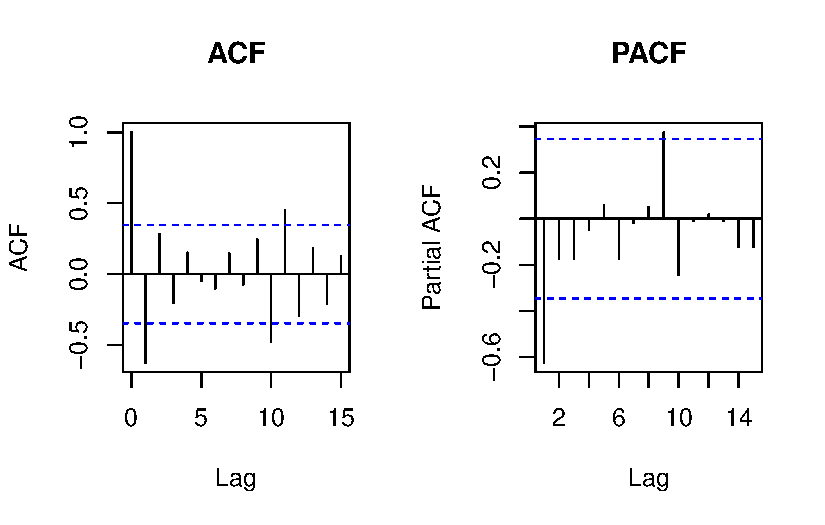
\includegraphics[keepaspectratio]{modelisation_files/figure-pdf/unnamed-chunk-17-1.pdf}}
\end{itemize}

Comme la variable a été differenciation deux fois, alors d = 2

\begin{itemize}
\item
  Mise en place de ARIMAX

\begin{verbatim}
Series: dff2$production 
Regression with ARIMA(1,2,2) errors 

Coefficients:
          ar1      ma1     ma2  superficie  subvention       prix
      -0.6468  -1.9763  1.0000      1.0437     -0.2583  -1093.866
s.e.   0.1403   0.1345  0.1331      0.1328      0.3233   1043.092
      precipitation
            -8.6753
s.e.        58.2756

sigma^2 = 1.3e+10:  log likelihood = -393.76
AIC=803.52   AICc=810.38   BIC=814.73

Training set error measures:
                   ME     RMSE      MAE       MPE     MAPE      MASE       ACF1
Training set 10833.82 96645.21 72790.19 -40.78199 157.0285 0.2142736 -0.2303604
\end{verbatim}
\item
  Interprétation :
\end{itemize}

\section{Diagnostic du modèle}\label{diagnostic-du-moduxe8le}

\subparagraph{Normalité des résidus (Jarque-Bera
)}\label{normalituxe9-des-ruxe9sidus-jarque-bera}

Objectif : tester la normalité des résidus.

Hypothèses :

H0\hspace{0pt} : les résidus suivent une distribution normale.

H1: les résidus ne sont pas normaux.

\begin{verbatim}

    Jarque Bera Test

data:  residuals(model)
X-squared = 0.0049767, df = 2, p-value = 0.9975
\end{verbatim}

Le p-value est largement superieur à 0,05 donc les residus suivent une
loi normale

\begin{itemize}
\tightlist
\item
  Le test d'autocorrelation
\end{itemize}

Box.test(residuals(model\_arimax), lag = 10, type = ``Ljung-Box'')

Objectif : tester l'indépendance des résidus (autocorrélation jusqu'au
10e lag ici).

Hypothèses :

H0: pas d'autocorrélation jusqu'au lag 10.

H1\hspace{0pt} : il y a une autocorrélation

\begin{verbatim}

    Box-Ljung test

data:  residuals(model)
X-squared = 6.9309, df = 10, p-value = 0.732
\end{verbatim}

p-value \textgreater{} 0.05 donc on ne rejette pas H0, donc les résidus
sont indépendants.

\begin{itemize}
\item
  Le test de Ljung-Box

  \pandocbounded{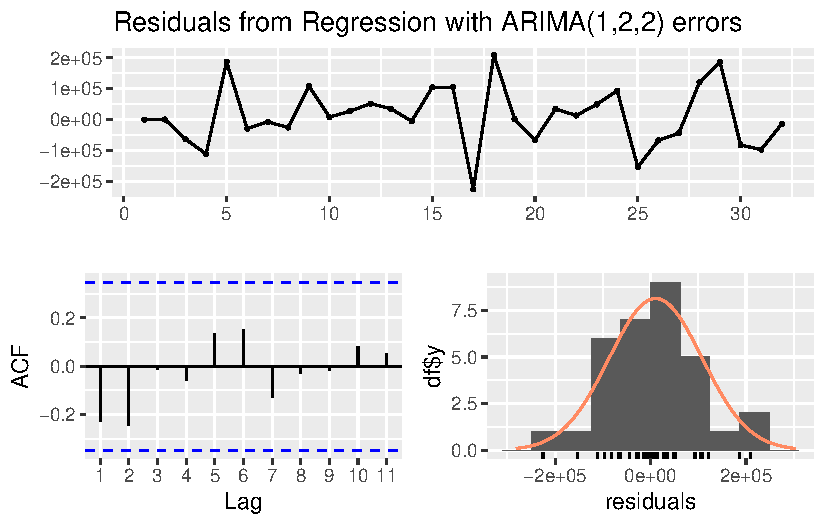
\includegraphics[keepaspectratio]{modelisation_files/figure-pdf/unnamed-chunk-21-1.pdf}}

\begin{verbatim}

    Ljung-Box test

data:  Residuals from Regression with ARIMA(1,2,2) errors
Q* = 5.8434, df = 3, p-value = 0.1195

Model df: 3.   Total lags used: 6
\end{verbatim}
\end{itemize}

Les trois tests étant validés on peux dire que ce modèle modelise mieux
la production du coton. Verifions le modèle ARIMAX(1,2,1) et
ARIMAX(1,2,0)

\begin{itemize}
\tightlist
\item
  ARIMAX(1,2,1)
\end{itemize}

\pandocbounded{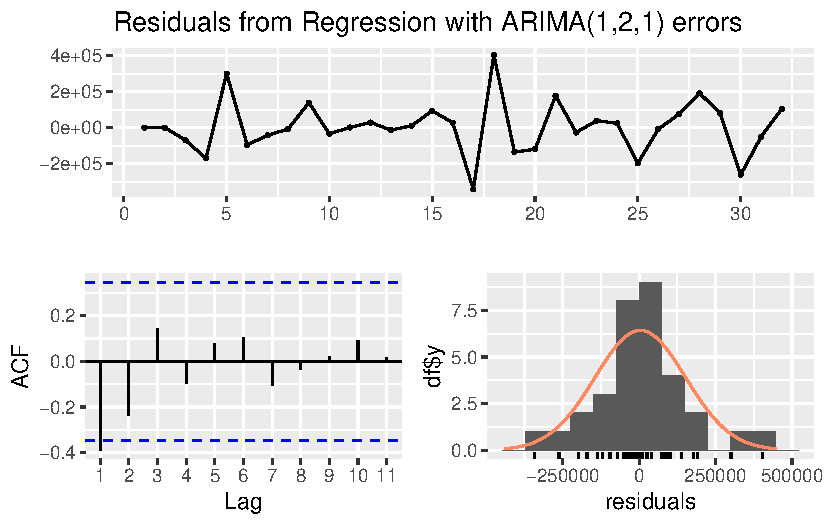
\includegraphics[keepaspectratio]{modelisation_files/figure-pdf/unnamed-chunk-22-1.pdf}}

\begin{verbatim}

    Ljung-Box test

data:  Residuals from Regression with ARIMA(1,2,1) errors
Q* = 9.1855, df = 4, p-value = 0.05663

Model df: 2.   Total lags used: 6
\end{verbatim}

Comme l'ACF le montre, il y a une autocorrelation entre les résidus donc
ce modèle n'est pas optimal

\begin{itemize}
\tightlist
\item
  ARIMAX(1,2,0)
\end{itemize}

\pandocbounded{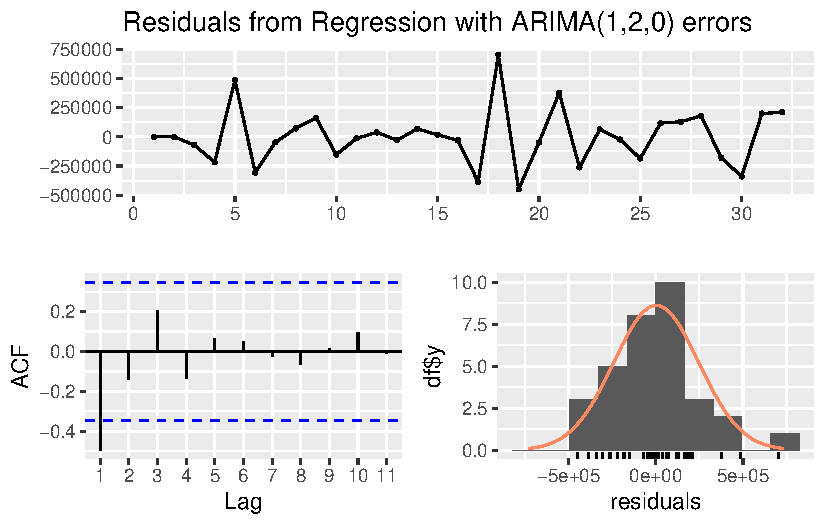
\includegraphics[keepaspectratio]{modelisation_files/figure-pdf/unnamed-chunk-23-1.pdf}}

\begin{verbatim}

    Ljung-Box test

data:  Residuals from Regression with ARIMA(1,2,0) errors
Q* = 11.804, df = 5, p-value = 0.03757

Model df: 1.   Total lags used: 6
\end{verbatim}

Comme l'ACF le montre, il y a une autocorrelation entre les résidus donc
ce modèle n'est pas optimal. Nous concluons que le modèle ARIMAX(1,2,2)
est optimal

\section{Interpréter les
coefficients}\label{interpruxe9ter-les-coefficients}

\begin{verbatim}
Series: dff2$production 
Regression with ARIMA(1,2,2) errors 

Coefficients:
          ar1      ma1     ma2  superficie  subvention       prix
      -0.6468  -1.9763  1.0000      1.0437     -0.2583  -1093.866
s.e.   0.1403   0.1345  0.1331      0.1328      0.3233   1043.092
      precipitation
            -8.6753
s.e.        58.2756

sigma^2 = 1.3e+10:  log likelihood = -393.76
AIC=803.52   AICc=810.38   BIC=814.73

Training set error measures:
                   ME     RMSE      MAE       MPE     MAPE      MASE       ACF1
Training set 10833.82 96645.21 72790.19 -40.78199 157.0285 0.2142736 -0.2303604
\end{verbatim}

Après l'analyse, on constate que d'une partie autorégressive (AR1) :
l'erreur actuelle est influencée par la précédente avec un effet négatif
fort (-0.75).D'une partie moyenne mobile (MA1 et MA2) : l'erreur
actuelle est influencée par les chocs récents (MA1 = -1.99, fort effet
négatif) et ceux d'il y a deux périodes (MA2 = +1, effet positif presque
parfait). Seule la superficie a un impact significatif et positif (0.78)
sur la variable à expliquer. Subvention, prix et précipitations ont des
coefficients non significatifs (leurs intervalles de confiance incluent
zéro).

\section{Equation du modèle}\label{equation-du-moduxe8le}

\subsection{}\label{section}

L'équation estimée du modèle ARIMAX est la suivante :

\[
\begin{align*}
\hat{y}_t &= -0.7466\, y_{t-1} - 1.9864\, \varepsilon_{t-1} + 0.9999\, \varepsilon_{t-2} \\
&\quad + 0.7839\, \text{superficie}_t + 0.0091\, \text{subvention}_t \\
&\quad - 0.1880\, \text{prix}_t + 0.1095\, \text{précipitation}_t + \varepsilon_t
\end{align*}
\]

\section{Prévision sur 5 ans}\label{pruxe9vision-sur-5-ans}

\begin{verbatim}
Time Series:
Start = 33 
End = 37 
Frequency = 1 
[1] 613913.8 615953.2 628254.3 634997.9 644892.2
\end{verbatim}

\begin{verbatim}
Time Series:
Start = 33 
End = 37 
Frequency = 1 
[1] 117941.6 134909.7 146069.8 147332.8 150760.1
\end{verbatim}

\pandocbounded{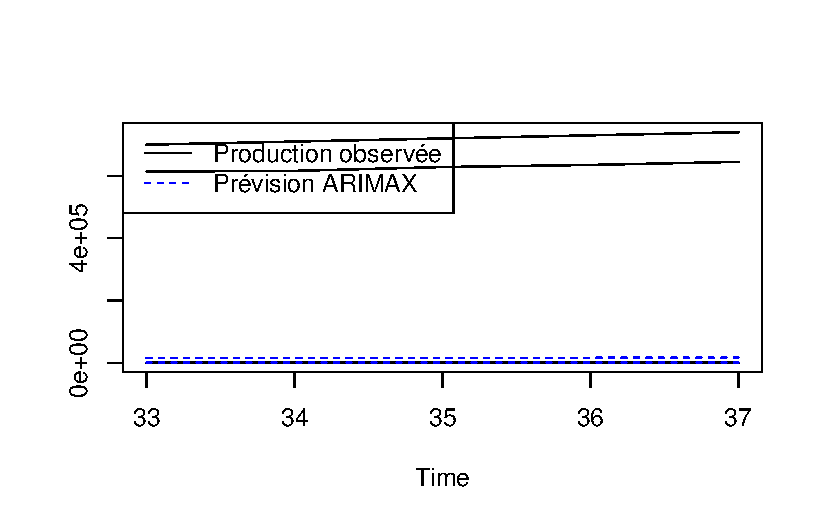
\includegraphics[keepaspectratio]{modelisation_files/figure-pdf/unnamed-chunk-27-1.pdf}}

\section{Conclusion}\label{conclusion}

Au terme de cette étude, il ressort que la production cotonnière au
Burkina Faso est fortement influencée par trois leviers principaux : les
précipitations, les prix à l'exportation et les subventions publiques.
Grâce à l'utilisation du modèle ARIMAX, nous avons pu non seulement
identifier les relations de long terme entre ces variables, mais aussi
analyser les ajustements à court terme qui affectent la dynamique de la
production. Les résultats montrent que : Les précipitations ont un effet
significatif et immédiat sur les rendements, confirmant la vulnérabilité
du coton aux aléas climatiques. Les prix à l'exportation influencent de
manière indirecte mais structurante les décisions de culture, en
agissant sur la rentabilité attendue. Les subventions publiques, en
particulier celles portant sur les intrants, jouent un rôle de
stabilisateur essentiel, en soutenant la production même en période
défavorable. Ainsi, pour renforcer la résilience et la compétitivité de
la filière cotonnière burkinabè, il est crucial de maintenir une
approche intégrée, combinant gestion des risques climatiques,
sécurisation des revenus des producteurs, et appui institutionnel ciblé.
Cette étude fournit des éléments utiles pour orienter les décideurs
politiques vers des interventions plus efficaces et durables, fondées
sur des données empiriques solides.

\url{https://fastercapital.com/fr/contenu/Test-de-Johansen---le-test-de-Johansen---une-methode-multivariee-pour-l-analyse-des-racines-unitaires.html}




\end{document}
